\documentclass{hw}
\usepackage{mhchem}
\usepackage{nuc}
\usepackage[load=addn]{siunitx}
\usepackage{amsmath}
\usepackage{cancel}
\usepackage{physics}
\graphicspath{ {images/}}

\author{J.R. Powers-Luhn}
\date{2016/10/20}
\title{Homework Chapters 5 and 6}

\begin{document}

\problem{Anderson 5.9}
A narrow beam of gamma rays passes through \SI{2.0}{\centi\meter} of lead. The incident beam consists of 30\% \SI{0.4}{\mega\electronvolt} photons and 70\% \SI{1.5}{\mega\electronvolt} photons. What fraction of the incident fluence is transmitted? Use Figure 5.5.

In addition to what's asked for in the question, find the effective attenuation coefficient.

\solution

\problem{Anderson 5.10}
A narrow beam of neutrons passes through \SI{2.0}{\centi\meter} of cadmium. The incident beam consists of 60\% \SI{0.02}{\mega\electronvolt} neutrons and 40\% \SI{0.5}{\mega\electronvolt} neutrons. What fraction of the incident fluence is transmitted? Use the information on Figure 5.6.

\solution

\problem{Anderson 5.14}
Calculate the dose for a \SI{100}{\roentgen} exposure measured in muscle tissue and bone at \SI{18}{\kilo\electronvolt} ($\ce{Mo}-\ce{K_\alpha}$), \SI{140}{\kilo\electronvolt} (\ce{^{99m}Tc}), and \SI{1.25}{\mega\electronvolt} (\ce{^{60}Co}) from the information on Figure 5.14. Assume that electronic equilibrium holds at the point of consideration.

\solution

\problem{}
Calculate the flux of epithermal neutrons needed to deliver a dose rate of \SI{0.1}{\gray\per\second} to muscle (tissue). Use an energy of \SI{0.1}{\mega\electronvolt} to represent the average energy of epithermal neutrons.

\solution

\problem{Anderson 6.4}
What is the angle of scatter and the energy of a Compton electron when the incident photon energy is \SI{140}{\kilo\electronvolt} and the angle of scatter of the photon is \SI{60}{\degree}?

\solution

\problem{}
Calculate the Compton edge energies (max scattered electron energy) for the following isotopes:
\begin{enumerate}
	\item $\ce{^{54}Mn}$
	\item $\ce{^{137}Cs}$
	\item $\ce{^{22}Na}$ (ignore the positron annihilation gammas)
\end{enumerate}

\solution

\problem{}
Using the photon energy from a $\ce{^{137}Cs}$ decay, calculate the following:
\begin{enumerate}
	\item The Klein Nishina total scattering cross section
	\item The total atomic cross section for Compton scattering in lead
	\item The Compton scattering attenuation coefficient in lead
\end{enumerate}

\solution

Please see attached code

\part

\begin{align*}
\sigma_{KN} &= \pi r_0^2 \left[ \frac{2\left(1 + \alpha \right)}{\alpha^2}\left( \frac{2\left(1+\alpha\right)}{1+2\alpha} - \frac{ln\left(1+2\alpha\right)}{\alpha}\right)+\frac{
\ln\left(1+2\alpha\right)}{\alpha}-\frac{2\left(1+3\alpha\right)}{\left(1+2\alpha\right)^2} \right] \\
\sigma_{KN} &= \SI{0.256}{\barn}
\end{align*}

\part

\begin{align*}
	\sigma_{compton} &= Z \sigma_{KN} \\
	\sigma_{compton} &= \SI{21}{\barn}
\end{align*}

\part

\begin{align*}
	\left( \frac{\mu}{\rho} \right)_{is} &= n_m \sigma_{is} \\
	\mu_{is} &= \frac{N_A Z}{M_m} \rho \sigma_{is} \\
	\mu_{is} &= \SI{56.78}{\per\centi\meter}
\end{align*}

\problem{}
Calculate the values for $\dv{\sigma_{KN}}{T_e}$ versus $T_e$ assuming an incoming photon energy of \SI{0.5}{\mega\electronvolt}. Calculate the values between $T_e=0$ and $T_e=T_{max}$ in step sizes of \SI{0.02}{\mega\electronvolt}. Plot your results and compare with figure 6.7

\solution
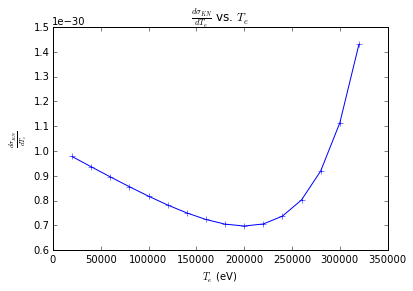
\includegraphics{551_6_8}

This strongly resembles figure 6.7, though without the vertical edge drawn in.

\end{document}